\DiaryEntry{Arithmetic Coding}{2021-05-19}{Coding}

In entry \ref{2021-05-11:entry} we have shown that collecting several symbols into one "super symbol" yields more efficient codes as we come close to the Shannon bound. 

This becomes impractical when we try to obtain Huffman codes for long sequences of symbols. In order to find the Huffman codeword for a particular sequence of length $m$, we need codewords for \emph{all} possible sequences of length $m$. This fact causes an exponential growth in the size of the codebook and makes Huffman coding impractical.

Instead, we need a way of assigning codewords to particular sequences without having to generate codes for all sequences of that length. The arithmetic coding technique fulfills this requirement. Here, a unique identifier or tag is generated for the sequence to be encoded. This tag corresponds to a binary fraction, which becomes the binary code for the sequence.

In practice, the generation of the tag and the binary code are the same process. However, the arithmetic coding approach is easier to understand if we conceptually divide the approach into two phases. In the first phase, a unique identifier or tag is generated for a given sequence of symbols. This tag is then given a unique binary code. A unique arithmetic code can be generated for a sequence of length $m$ without the need for generating codewords for all sequences of length $m$.

\subsection{Basic idea}

In order to distinguish a sequence of symbols from another sequence of symbols we need to tag it with a unique identifier. One possible set of tags for representing sequences of symbols, are the numbers in the unit interval $[0, 1)$. Because the number of numbers in the unit interval is infinite, it should be possible to assign a unique tag to each distinct sequence of symbols. In order to do this, we need a function that will map sequences of symbols into the unit interval. A function that maps random variables, and sequences of random variables, into the unit interval is the cumulative distribution function (cdf) of the random variable associated with the source. This is the function we will use in developing the arithmetic code.

If symbol $a_i$ is emitted from the source with probability $P(X = a_i)$, then the corresponding cdf is defined as

\bee
F_X(i) = \sum_{k=1}^i P(X = k)
\eee

Note that for each symbol $a_i$ with a nonzero probability, we have a distinct value of $F_X(i)$.

\subsection{Tag Generation}

The tag of a sequence is any number in the interval bounded by the cdf of the sequence and the cdf of the sequence preceding it in some agreed upon ordering. The procedure for generating the tag works by reducing the size of the interval in which the tag resides as more and more elements of the sequence are received.

We start out by first dividing the unit interval into subintervals of the form $[F_X(i - 1), F_X(i)], i = 1, \ldots, m$. This partitions the unit interval as the cdf lies in the unit interval. We associate the subinterval $[F_X(i - 1), F_X (i)]$ with the symbol $a_i$ . The appearance of the first symbol in the sequence restricts the interval containing the tag to one of these subintervals. Suppose the first symbol was $a_k$. Then the interval containing the tag value will be the subinterval 

\bee
\left[ F_X(k-1), F_X(k) \right]
\eee

For the next symbol, this subinterval is now partitioned in the same proportions as the original interval. So if the second symbol in the sequence is $a_j$, then the interval containing the tag value becomes 

\bee
\left[ F_X(k - 1) + \frac{F_X(j - 1)}{F_X(k) - F_X(k - 1)}, F_X(k - 1) + \frac{F_X(j)}{F_X(k) - F_X(k - 1)} \right]
\eee

Each succeeding symbol causes the tag to be restricted to a subinterval that is further partitioned in the same proportions.

\paragraph{Example.} We use a three-symbol alphabet $\Sc = \{a_1, a_2, a_3\}$ with symbol probabilities $P(a_1) = 0.7, P(a_2) = 0.1, P(a_3) = 0.2$. The cdf is therefore $F_X(1) = 0.7, F_X(2) = 0.8, F_X(3) = 1$. The partitioning of the unit interval for the first sybmol to be encoded is shown in the left part of the following Figure. If symbol $a_1$ needs to be encoded, the corresponding tag lies within $[0, 0.7]$, if $a_2$ needs to be encoded, the corresponding tag lies within $[0.7, 0.8]$, and if $a_3$ needs to be encoded, the corresponding tag lies within $[0.8, 1.0]$. For the example, we assume that we decode $a_1$; therefore the tag lies in $[0, 0.7]$.

We now split the interval $[0, 0.7]$ proportionally; this is shown in the middle of the following Figure. Assuming that our second symbol to encode is $a_2$, the corresponding tag lies now in $[0.49, 0.56]$. Note that this is the tag for the \emph{complete sequence}.

Finally decoding $a_3$, we see that the tag is now restricted to the interval $[0.546, 0.560]$. This is shown in the right part of the following Figure.

\begin{figure}[H]
    \centering
    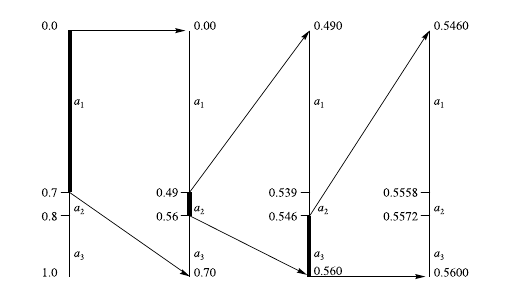
\includegraphics[scale=0.7]{images/2021-05-19-arith_coding_1.png}
  \end{figure}
  
The example shows that the more symbols we receive, the smaller our interval becomes. Moreover, the intervals are non-overlapping; i.e. were the first symbol different, then our final interval for the tag would be a completely different non-overlapping interval. This shows thatt we can use any value from the interval for the tag; in the following, we will use the interval midpoint. \qed

The interesting thing is that we can compute the interval for the $n$-th symbol recursivley as we receive one symbol after the other. Denote the interval of the $n$-th symbol by $[l^{(n)}, u^{(n)}]$, we have

\begin{align}\label{2021-05-18:eq1}
    l^{(n)} &= l^{(n-1)} + (u^{(n-1)}) - l^{(n-1)}) F_X(x_n-1) \\
    u^{(n)} &= l^{(n-1)} + (u^{(n-1)}) - l^{(n-1)}) F_X(x_n)
\end{align}

Initial values are $l^{(0)} = 0, u^{(0)} = 1$.

Let's try this with our example. For the first symbol $a_1$ we have the following interval bounds

\begin{align*}
    l^{(1)} &= l^{(0)} + (u^{(0)}) - l^{(0)}) F_X(0) = 0 + (1 - 0) 0 = 0 \\
    u^{(1)} &= l^{(0)} + (u^{(0)}) - l^{(0)}) F_X(1) = 0 + (1 - 0) 0.7 = 0.7
\end{align*}

as $F_X(0) = 0$. So the tag for $a_1$ lies in the interval $[0, 0.7]$. We next decode $a_2$, this yields the following new interval bounds

\begin{align*}
    l^{(2)} &= l^{(1)} + (u^{(1)}) - l^{(1)}) F_X(2-1) = 0 + (0.7 - 0) 0.7 = 0.49 \\
    u^{(2)} &= l^{(1)} + (u^{(1)}) - l^{(1)}) F_X(2) = 0 + (0.7 - 0) 0.8 = 0.56
\end{align*}

and therefore our tag must be in $[0.49, 0.56]$. Decoding $a_3$ we update our bounds to

\begin{align*}
    l^{(3)} &= l^{(2)} + (u^{(2)}) - l^{(2)}) F_X(2) = 0.49 + (0.56 - 0.49) 0.8 = 0.546 \\
    u^{(3)} &= l^{(2)} + (u^{(2)}) - l^{(2)}) F_X(3) = 0.49 + (0.56 - 0.49) 1 = 0.56
\end{align*}

and the tag lies within $[0.546, 0.56]$. Comparing this with the Figure above, we see that the values match.

For now, we choose the interval midpoint $0.533$ as tag value.

\subsection{Decoding Tags}

Now we go the other direction: We receive a tag and want to reconstruct the sequence of symbols the tag represents. For every symbol received, we need to calculate the bounds $l^{(n)}$ and $u^{(n)}$ for all symbols $n$ and decide in which interval the received tag falls into.

More formally, we have the following algorithm for decoding a given tag $T$.

\begin{enumerate}
    \item Initialize $l^{(0)} = 0, u^{(0)} = 1, k=1$.
    \item Calculate $t_k^\star = \frac{T - l^{(k-1)}}{u^{(k-1)} - l^{(k-1)}}$.
    \item Find the value of $x_k$ for which $F_X(x_k-1) \leq t_k^\star \leq F_X(x_k)$ and output the corresponding symbol.
    \item Update $l^{(k)}, u^{(k)}$ based on the chosen $x_k$.
    \item Set $k = k+1$ and repeat from step $2$ until the entire sequence is decoded.
\end{enumerate}

\paragraph{Example.} We continue with our running example with tag $T = 0.553$. We get $t_1^\star = 0.553$ and this falls into the first interval $[0, 0.7]$. Therefore, the first symbol is $a_1$. From this, we update $l^{(1)} = 0, u^{(1)} = 0.7$ and continue with $k=2$.

We have $t_1^\star = 0.79$; this falls into the second interval $[0.7, 0.8]$, therefore the second symbol is $a_2$. We yield a new interval as $[0.49, 0.56]$.

We have $t_2^\star = 0.9$ which is in the third interval $[0.8, 1]$, therefore the third symbol is $a_3$ and we are done. \qed

There are two ways to know when the entire sequence has been decoded. The decoder may know the length of the sequence, in which case the deciphering process is stopped when that many symbols have been obtained. The second way to know if the entire sequence has been decoded is that a particular symbol is denoted as an  end-of-transmission symbol. The decoding of this symbol would bring the decoding process to a close.

\subsection{Practical Issues / Outlook}

Using the algorithms described so far, we can obtain a tag for a given symbol sequence. However, the \emph{binary code} for the sequence is what we really want to know (and we want to find it in a unique and efficient manner). 

We have said that the tag forms a unique representation for the sequence. This means that the binary representation of the tag forms a unique binary code for the sequence. However, we have placed no restrictions on what values in the unit interval the tag can take. The binary representation of some of these values would be infinitely long, in which case, although the code is unique, it may not be efficient. To make the code efficient, the binary representation has to be truncated. But if we truncate the representation, is the resulting code still unique? Finally, is the resulting code efficient? How far or how close is the average number of bits per symbol from the entropy?

In practice, the number of numbers that can be uniquely represented on a machine is limited by the maximum number of digits (or bits) we can use for representing the number. We have seen that the update interval equations \ref{2021-05-18:eq1} cause the intervals to become smaller and smaller. This means that in order to represent all of the subintervals uniquely, we need increasing precision as the length of the sequence increases. In a system with finite precision, the two values are bound to converge; and we will lose all information about the sequence from the point at which the two values converged. To avoid this situation, we need to rescale the interval. However, we have to do it in a way that will preserve the information that is being transmitted. We would also like to perform the encoding incrementally - that is, to transmit portions of the code as the sequence is being observed, rather than wait until the entire sequence has been observed before transmitting the first bit.

The solution to these practical considerations will be described in a future post.






%%% Local Variables:
%%% mode: latex
%%% TeX-master: "journal"
%%% End:
